\section{Generating the Path}

The MPC application expects a parameterized path that can be either linear or curved. The linear paths will be generated using parameterization, and the curved paths will be generated as Dubins paths. This will be done using Matlab, and the generated paths will be stored in a text file containing only the points on the path.

One important matter when generating the paths is to ensure that the resolution of the path is high enough. How high the resolution needs to be depends on the speed of aircraft and the length of the timestep, and how much uncertainty is accepted when generating the trajectory. 


\subsubsection{Dubins Path}

A Dubins path is a path that consists of two circles connected by a straight line, and it has been proven that this is the shortest path between two vehicle configurations \cite{DUBINS}. In order to generate the Dubins path the algorithms presented by Beard \& McLain \cite{uavBEARD} will be used. An illustration of a simple Dubins path is shown in figure \ref{fig:dubins}.

\begin{figure}[h]
	\centering
    \makebox[\textwidth][c]{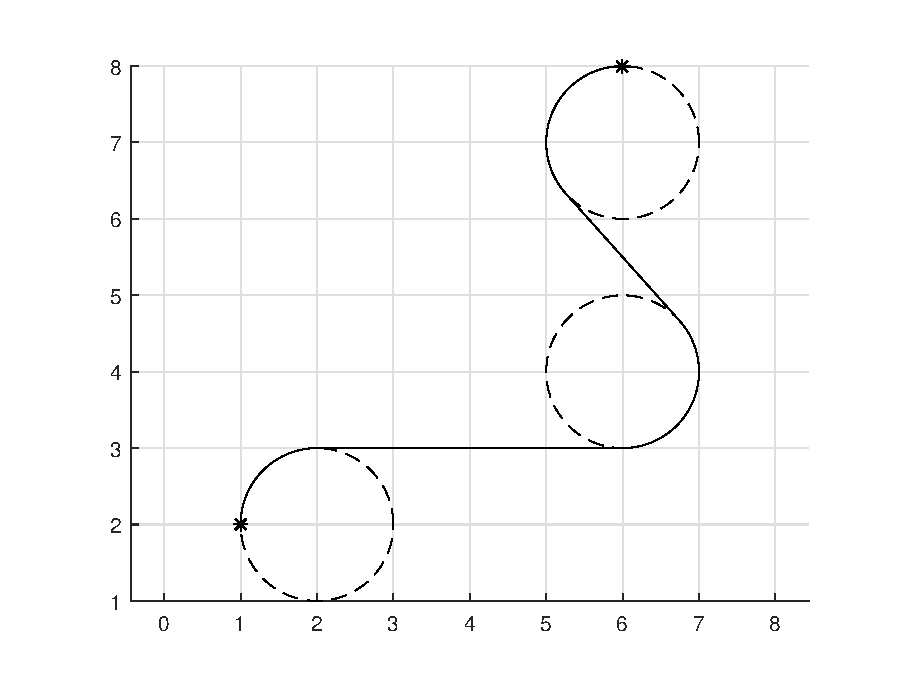
\includegraphics[width=\textwidth, keepaspectratio=true]{dubins_example.eps}}
	\caption{An illustration of a simple Dubins path.}
	\label{fig:dubins}
\end{figure}